% Shared standalone design for the editable figure reconstructions.
\documentclass[tikz,border=5pt,10pt]{standalone}
\usepackage[T1]{fontenc}
\usepackage[utf8]{inputenc}
\usepackage{newpxtext,newpxmath}
\usepackage[scaled=.94]{sourcesanspro}
\usepackage{pgfplots}
\pgfplotsset{compat=1.18}
\usetikzlibrary{arrows.meta,calc,positioning,decorations.pathreplacing,
  decorations.markings,patterns,matrix,shapes.geometric,fit,backgrounds,
  intersections,angles,quotes}
\definecolor{ink}{HTML}{203746}
\definecolor{accent}{HTML}{146C78}
\definecolor{muted}{HTML}{667780}
\definecolor{signalred}{HTML}{B94B44}
\color{ink}
\tikzset{>=Latex,line width=.8pt,
  every node/.style={font=\small},
  axis/.style={->,draw=muted,line width=.5pt},
  guide/.style={draw=muted,dashed,line width=.45pt},
  curve/.style={draw=accent,line width=1pt},
  marker/.style={circle,fill=accent,inner sep=1.5pt},
  labelbox/.style={fill=white,inner sep=2pt}}

\begin{document}
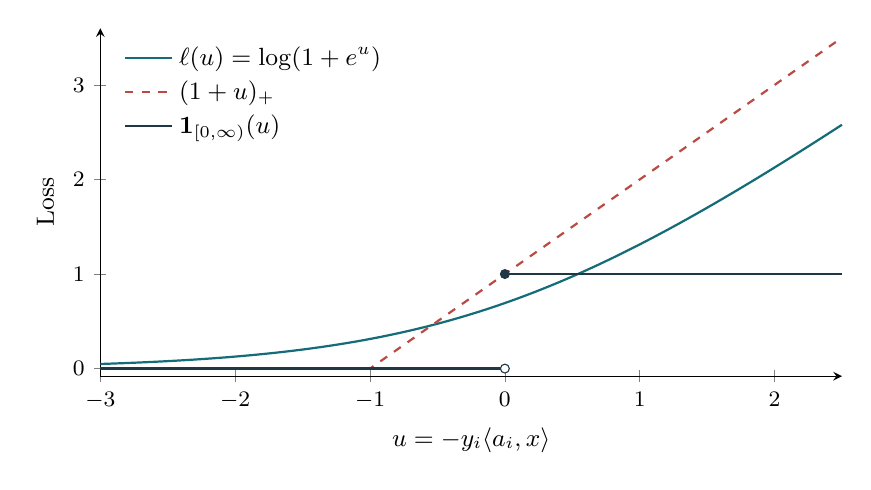
\begin{tikzpicture}
\begin{axis}[width=11cm,height=6cm,xmin=-3,xmax=2.5,ymin=-.08,ymax=3.6,axis lines=left,xlabel={$u=-y_i\langle a_i,x\rangle$},ylabel={Loss},xtick={-3,-2,-1,0,1,2},ytick={0,1,2,3},tick label style={font=\footnotesize},legend style={at={(.02,.98)},anchor=north west,draw=none,fill=white,font=\small},legend cell align=left,clip=false]
\addplot[accent,thick,domain=-3:2.5,samples=120] {ln(1+exp(x))};\addlegendentry{$\ell(u)=\log(1+e^u)$}
\addplot[signalred,dashed,thick,domain=-3:2.5,samples=100] {max(0,1+x)};\addlegendentry{$(1+u)_+$}
\addplot[ink,thick] coordinates {(-3,0) (0,0)};\addlegendentry{$\mathbf{1}_{[0,\infty)}(u)$}
\addplot[ink,thick,forget plot] coordinates {(0,1) (2.5,1)};
\addplot[only marks,mark=*,mark size=1.6pt,ink,forget plot] coordinates {(0,1)};
\addplot[only marks,mark=*,mark size=1.6pt,mark options={fill=white,draw=ink},forget plot] coordinates {(0,0)};
\end{axis}
\end{tikzpicture}
\end{document}
